\documentclass[10pt]{article}

% Pacotes extras necessários
\usepackage{amsmath}
\usepackage[lmargin=0.5in, rmargin=0.5in, tmargin=0.5in, bmargin=0.5in, includehead, includefoot]{geometry}
\usepackage{amsfonts}
\usepackage[utf8]{inputenc}
\usepackage[portuguese]{babel}
\usepackage{graphicx}
\usepackage{fancyhdr}
\usepackage{setspace}
\usepackage{listings}
\usepackage{url}
\usepackage{enumitem}
\usepackage{appendix} % For creating appendix sections

% More defined colors
\usepackage[dvipsnames]{xcolor}

% Define a custom style for the code listing
\lstdefinestyle{mystyle}{
    language=Octave,
    backgroundcolor=\color{white},   % Choose the background color
    basicstyle=\ttfamily\footnotesize, % Set the font and size for the code
    numbers=left,                    % Line numbers on the left
    numberstyle=\tiny\color{gray},   % Line numbers style
    numbersep=5pt,                   % Distance of line numbers from the code
    tabsize=2,                       % Set tab size (default is 8 spaces)
    breaklines=true,                 % Automatically wrap long lines
    keywordstyle=\color{blue},       % Keywords in blue
    commentstyle=\color{green!60!black}, % Comments in green
    stringstyle=\color{orange},      % Strings in orange
    frame=single,                    % Draw a frame around the code
    keepspaces=true,                 % Preserve spaces in text
    showspaces=false,                % Don't show spaces in strings
    showstringspaces=false,          % Don't show spaces in strings
    showtabs=false,                  % Don't show tabs in strings
    % Add any other options you need
}

\lstset{style=mystyle} % Set the custom style
 
% Required package
\usepackage{tikz}
\usetikzlibrary{positioning}

\graphicspath{ {./images/} }

% Sets para outras partes
\setlength{\parindent}{0pt}
\setstretch{1.5}
\DeclareMathOperator{\sen}{sen}
\DeclareMathOperator{\sinc}{sinc}

%% Facilidades
%% -- Laplace
\newcommand{\Lap}[1]{\mathcal{L}\left\{#1\right\}}

%% -- Negrito em matemáticas
\newcommand{\bm}[1]{\boldsymbol{#1}}


% ------- Estilo do trabalho -------- %
\fancypagestyle{capa}{
    \fancyhf{}
    \renewcommand\headrulewidth{0pt}
}

\pagestyle{fancy}
\fancyhead{}
\fancyhead[L]{\thepage}
\fancyfoot{}
% ----------------------------------- %

% Dados do Grupo
\title{Modelagem de Sistemas Dinâmicos - Trabalho Nº4}
\author{
    Leonardo Soares da Costa Tanaka - DRE: 121067652 \\
    Engenharia de Controle e Automação/UFRJ \\
    Rio de Janeiro, Brasil \\
    Julho de 2023
}
\date{}

\begin{document}
\maketitle
\thispagestyle{capa}

\quad Para este trabalho, vamos utilizar o arquivo “trabalho4-2023-1.mat” que tem os sinais de entrada u(t) e de saída y(t) de um sistema
linear contínuo com função de transferência G(s). Os sinais u e y foram aplicados e aquisitados
com uma frequência de amostragem fs = 2Hz (período de amostragem T = 0.5s). A variável
independente tempo t é o vetor com os instantes que foram realizadas as amostragens dos
sinais u(t) e y(t).

\quad Vale notar que o sinal de saída y(t) está quantizado e contaminado com ruído.

\section{FFT}

\quad Determinando, utilizando a FFT (Fast Fourier Transform), o espectro do sinal de entrada
(módulo e fase) em função da frequência em Hz. Utilizando o Matlab para coletar os dados,
utilizar a FFT, calcular os espectros do sinal de entrada e plotar o gráfico.

\begin{figure}[h]
    \centering
    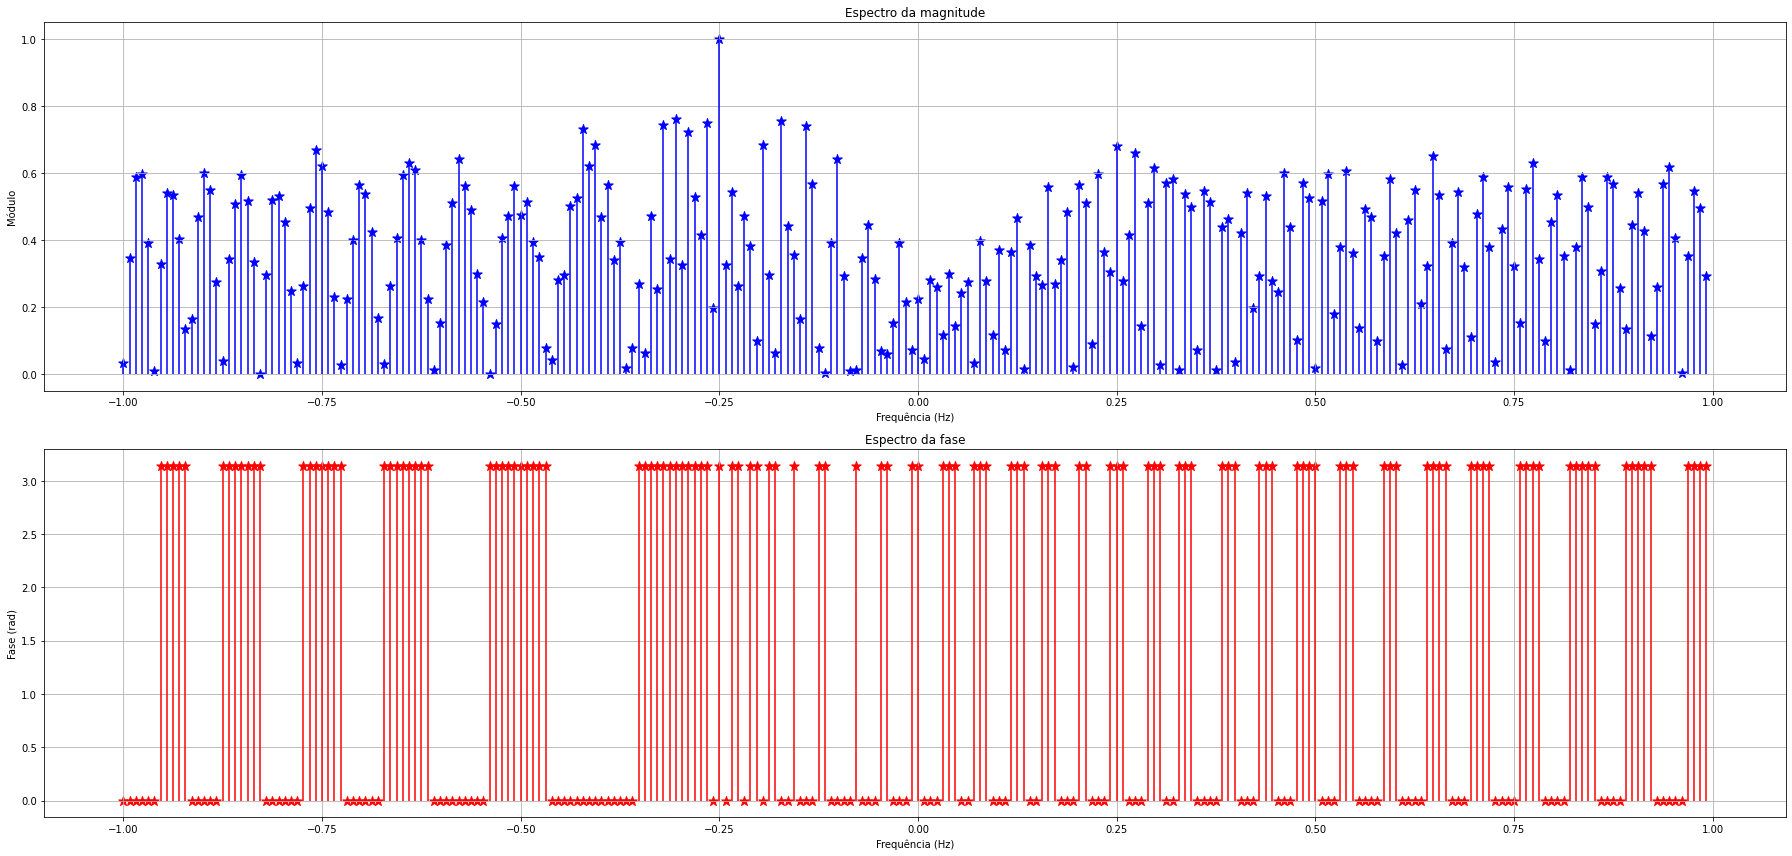
\includegraphics[scale=0.34]{fft.png}
    \caption{Espectros dos sinais da entrada}
\end{figure}

\quad É possível observar uma simetria no gráfico da mangnitude em torno de 1
com uma parte central com valores iguais a 2.61115 entre 0.4 e 1.6,
duas partes seguintes com valores iguais a 10.4446 entre (0.03 e 0.4) e (1.6 e 1.96) e duas
partes extremas com os mesmos valores que a parte central. Já no gráfico de fase, é possível
observar uma oscilação bem similar entre 0.4 e 1.6 e
outras oscilações similares entre (0.03 e 0.4) e (1.6 e 1.96) com valores entre $-\pi$ e $\pi$.

\small
\begin{verbatim}
    % Carregar os dados do arquivo
    data = load('trabalho4-2023-1.mat');
    u = data.u;
    t = data.t;
    % Frequência de amostragem (fs) e período de amostragem (T)
    fs = 2; % Hz
    T = 1 / fs;
    % Calcula o espectro do sinal de entrada u(t) usando a FFT
    U = fft(u);
    % Vetor de frequências para o eixo x
    frequencies = (0:length(U) - 1) * (fs / length(U));
    % Módulo do espectro do sinal de entrada
    modulo_U = abs(U);
    % Fase do espectro do sinal de entrada
    fase_U = angle(U);
    % Cores para os plots
    cor_modulo = 'b'; % Azul
    cor_fase = 'r';   % Vermelho
    % Plot do espectro do sinal de entrada (módulo e fase)
    figure;
    % Plot do módulo do espectro
    subplot(2, 1, 1);
    stem(frequencies, modulo_U, 'Color', cor_modulo);
    xlabel('Frequência (Hz)');
    ylabel('Módulo');
    title('Módulo do espectro do Sinal de Entrada u(t)');
    grid on;
    % Plot da fase do espectro
    subplot(2, 1, 2);
    stem(frequencies, fase_U, 'Color', cor_fase);
    xlabel('Frequência (Hz)');
    ylabel('Fase (rad)');
    title('Fase do Espectro do Sinal de Entrada u(t)');
    grid on;
\end{verbatim}

\section{Resposta em frequência do sistema G(jw)}

\quad Estimando a resposta em frequência do sistema G(jw) utilizando os espectros dos sinais
de entrada U(jw) e de saída Y(jw):

\begin{figure}[h]
    \centering
    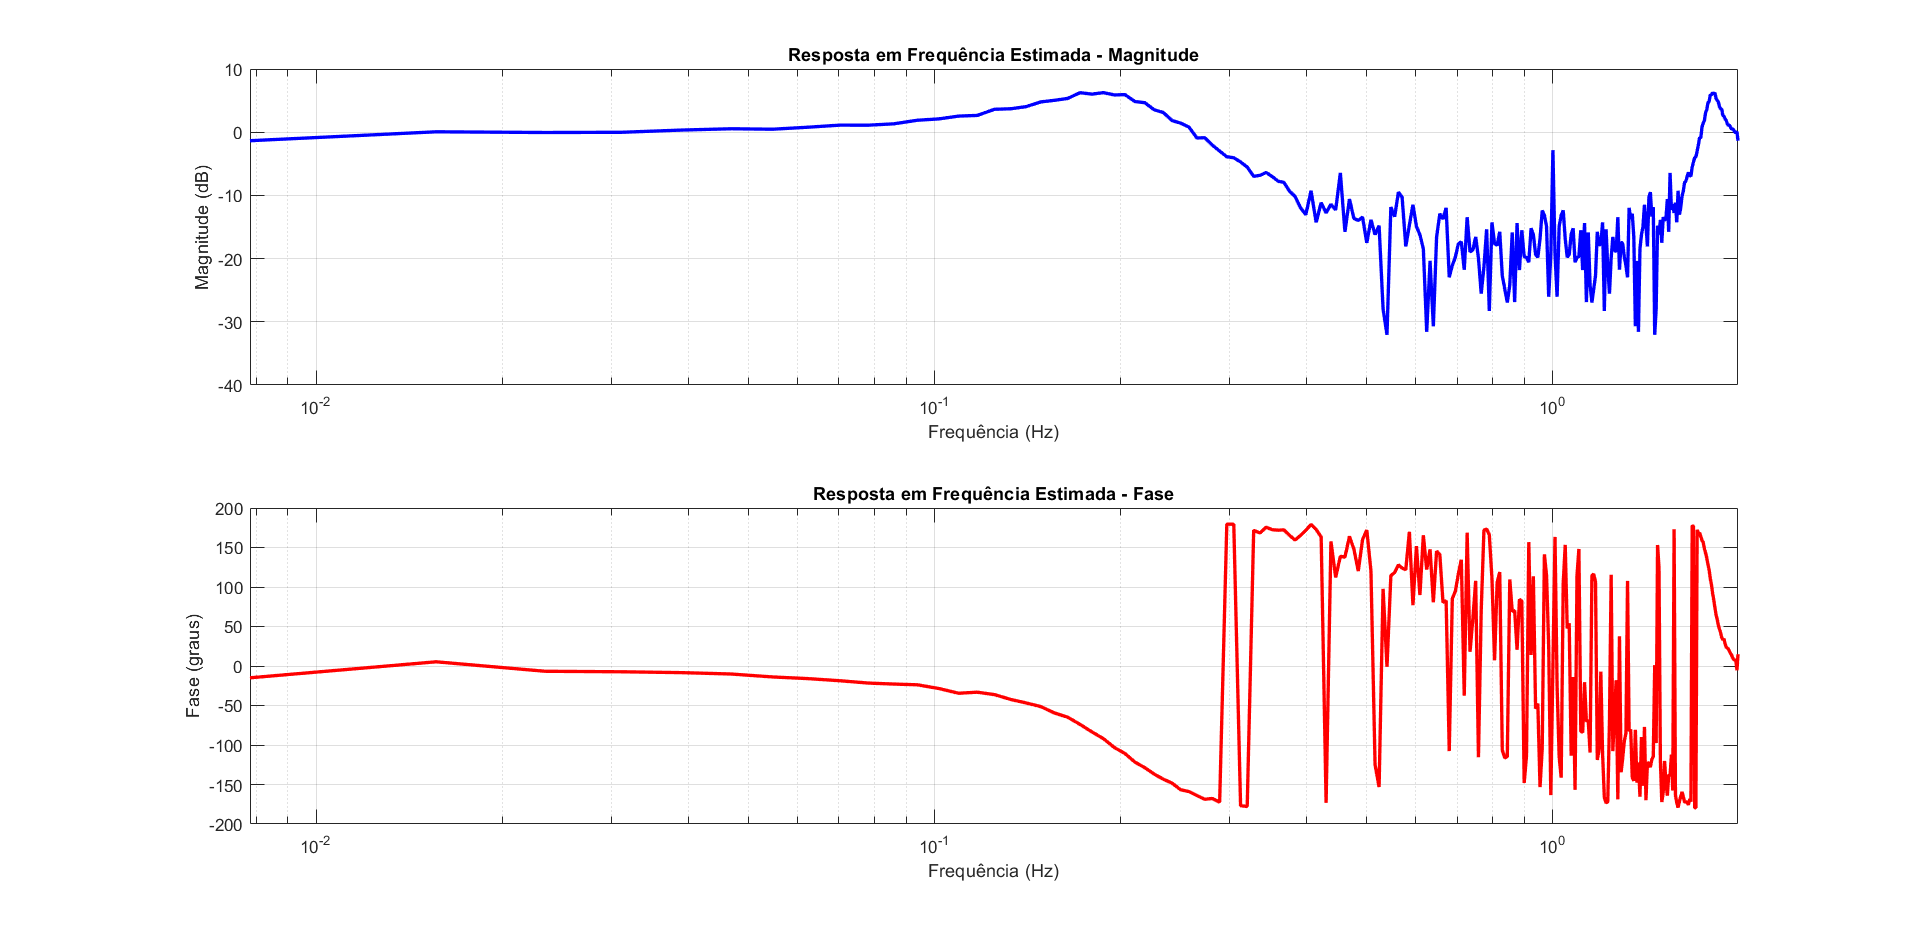
\includegraphics[scale=0.26]{g.png}
    \caption{Resposta em frequência}
\end{figure}

\small
\begin{verbatim}
    % Carregar o arquivo 'trabalho4-2023-1.mat'
    load('trabalho4-2023-1.mat');
    % Frequência de amostragem
    fs = 2; % Hz
    % Realizar a FFT do sinal de entrada 'u'
    U = fft(u);
    U_mag = abs(U);
    U_phase = angle(U);
    % Realizar a FFT do sinal de saída 'y'
    Y = fft(y);
    Y_mag = abs(Y);
    Y_phase = angle(Y);
    % Estimar a resposta em frequência do sistema G(jw)
    G_estimated = Y ./ U;
    G_mag_dB = 20*log10(abs(G_estimated));
    G_phase_deg = rad2deg(angle(G_estimated));
    % Frequências correspondentes
    N = length(u);
    frequencies = (0:N-1) * (fs/N);
    % Plotar o módulo e fase da resposta em frequência estimada na mesma figura em escala logarítmica
    figure;
    subplot(2, 1, 1);
    semilogx(frequencies, G_mag_dB, 'b', 'LineWidth', 2);
    title('Resposta em Frequência Estimada - Magnitude');
    xlabel('Frequência (Hz)');
    ylabel('Magnitude (dB)');
    grid on;
    subplot(2, 1, 2);
    semilogx(frequencies, G_phase_deg, 'r', 'LineWidth', 2);
    title('Resposta em Frequência Estimada - Fase');
    xlabel('Frequência (Hz)');
    ylabel('Fase (graus)');
    grid on; 
\end{verbatim}

\section{Principais caracteríticas da resposta em frequência}

\newpage

\section{Determinação do sistema de 2$\textsuperscript{a}$ ordem}

\section{System Identification Apps}

\end{document}